\chapter{Extended Language Models}

This chapter describes several recently proposed NLM architectures designed to tackle the rare word prediction problem and highlights the main similarities and differences among them. We also introduce our proposed model called ``Sentinel Mixture''.

\section{Attention Models}
\label{sec:attention}

Although the concept of attention that we are going to introduce is not directly concerned with rare word prediction, it will help us lay the foundations for the subsequent language models as they take inspiration from it.

\subsection{Original Formulation}

Attention models were firstly developed in the field of neural machine translation (NMT) in the seminal paper \cite{bahdanau2014neural}. At that time, most of the proposed NMT models belonged to a family known as ``encoder-decoders'' \cite{sutskever2014sequence}. These models consist of two parts: first an encoder (a deep bidirectional LSTM network) compresses the input sentence (specifically the embeddings for each word) $\{\mathbf{x}(1), \mathbf{x}(2), \cdots, \mathbf{x}(n_x)\}$ into a fixed-length vector representation $\mathbf{c}$. This is done by sequentially processing the sentence with a recurrent network and taking the last hidden state $\mathbf{h}(n_x)$ as $\mathbf{c}$ (\autoref{eq:encoder}).

\begin{equation} \label{eq:encoder}
	\begin{gathered}
		\mathbf{h}(t) = \text{LSTM}(\mathbf{x}(t), \mathbf{h}(t-1)) \\
		\mathbf{c} = \mathbf{h}(n_x)
	\end{gathered}
\end{equation}

Then a decoder (also a deep LSTM network) outputs a translation sentence $o=\{o(1), o(2), \cdots, o(n_o)\}$ using $\mathbf{c}$ as its initial hidden state. As shown in \autoref{eq:decoder}, in a similar way as the RNNLM that we saw in \autoref{sec:rnn}, the probability of outputting a word at step $t$ is obtained as the vocabulary softmax of an affine transformation of the hidden state $\mathbf{s}(t)$.

\begin{equation} \label{eq:decoder}
	\begin{gathered}
		\mathbf{s}(t) = \text{LSTM}(\mathbf{o}(t-1), \mathbf{s}(t-1)) \\
		p(o) = \prod_{t=1}^{n_o} p(o(t)|\{o(1), \cdots, o(t-1)\}, \mathbf{c}) \\
		p(o(t)|\{\mathbf{o}(1), \cdots, \mathbf{o}(t-1)\}, \mathbf{c}) = \text{softmax}(W_o \mathbf{s}(t) +\textbf{b}_o)
	\end{gathered}
\end{equation}

A potential problem for this architecture is the fact that all the necessary information from an input sentence has to be encoded into the vector $\mathbf{c}$. Hence, this may make it difficult for the model to deal with long sentences. Instead, an attention layer is added to give the decoder access to the full sequence of the encoder's hidden states $\{\mathbf{h}(1), \mathbf{h}(2), \cdots, \mathbf{h}(n_x)\}$, as shown in \autoref{fig:nmtAttention}.

\begin{figure}[H]
	\centering
	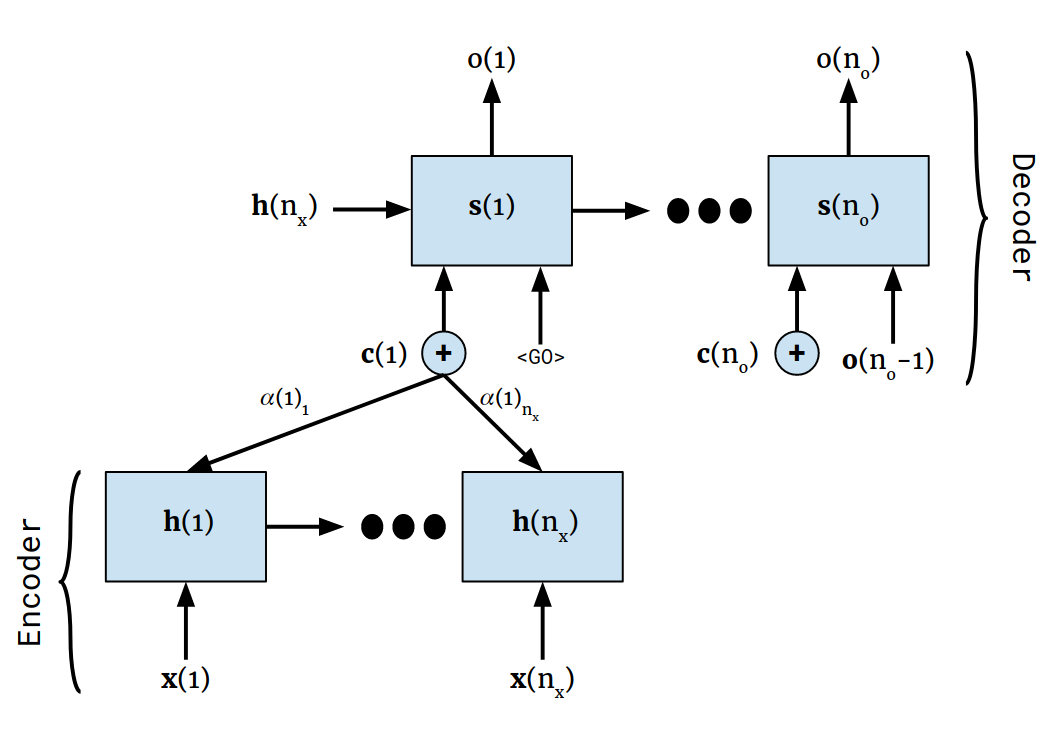
\includegraphics[scale=0.28]{nmt}
	\captionof{figure}{Attention NMT model.}
	\label{fig:nmtAttention}
\end{figure}

In this new architecture the decoder is provided with an additional input, the context vector $\mathbf{c}(t)$. For each step $t$ of the decoder, it is calculated in the following way:

\begin{equation} \label{eq:nmtAttention}
	\begin{gathered}
		e_{tk} = \mathbf{e}(t)_k = \mathbf{v_a}^{\top} \tanh(W_a \mathbf{s}(t-1)+U_a\mathbf{h}(k)), \; \forall k \in 1, \cdots , n_x  \\
		\alpha_{tk} = \boldsymbol{\alpha}(t)_k = \frac{e^{e_{tk}}}{\sum_{j}e^{e_{tj}}}, \; \forall k \in 1, \cdots , n_x  \\
		\mathbf{c}(t) = \sum_{k=1}^{n_x} \alpha_{tk} \mathbf{h}(k)
	\end{gathered}
\end{equation}

where $\mathbf{e}(t),\boldsymbol{\alpha}(t) \in \mathbb{R}^{n_x}$, $W_a \in \mathbb{R}^{h \times h}$, $U_a \in \mathbb{R}^{h \times 2h}$, $\mathbf{h}(t) \in \mathbb{R}^{2h}$ and $\mathbf{v_a},\mathbf{s}(t),\mathbf{c}(t) \in \mathbb{R}^{h}$. 

First, a vector of attention scores $\mathbf{e}(t)$ is calculated in order to see how much each input word should be ``attended'' with respect to the current decoder step. These are obtained with a single-layer multilayer perceptron. Next, the scores are normalized via a softmax operation producing the attention weights (can also be interpreted as probabilities)  $\boldsymbol{\alpha}(t)$. Finally, the context vector $\mathbf{c}(t)$ is obtained as a convex combination of all the encoder's hidden states weighted by $\boldsymbol{\alpha}(t)$.

\subsection{Types of Attention}

Since its introduction, attention has been applied successfully in other areas such as computer vision \cite{xu2015show} and adapted for many other NLP tasks. In this section we introduce one possible classification (inspired by \cite{luongeffective}) of such models attending to three different aspects:

\begin{itemize}
	\item  Depending on the attention's span:
		\begin{itemize}
			\itemsep 0em
			\item  \textbf{Global:} all inputs are taken into account.
			\item  \textbf{Local:} only a subset of all inputs is used.
		\end{itemize}
	\item  Depending on whether all inputs are allowed to contribute to the context:
		\begin{itemize}
			\itemsep 0em
			\item  \textbf{Soft:} context is built as a deterministic weighted combination of the inputs. This variant is smooth and differentiable so learning can be done by using standard backpropagation.
			\item  \textbf{Hard:} context is chosen as a single input that is selected stochastically. This has the drawback of requiring learning techniques such as Monte Carlo sampling or reinforcement learning.
		\end{itemize}
	\item  Depending on whether the content of inputs is used when computing the attention scores:
		\begin{itemize}
			\itemsep 0em
			\item  \textbf{Location-based:} the attention score for each input is obtained without taking into account their contents (e.g. $\mathbf{h}(t)$ in the setting described in the previous section).
			\item  \textbf{Content-based:} the input's contents are involved when calculating how relevant is each of them. This can be done in multiple ways and some examples are: dot product $\mathbf{s}(t)^{\top}\mathbf{h}(t)$, general $\mathbf{s}(t)^{\top}W\mathbf{h}(t)$ or ``concatenation'' $W\mathbf{s}(t) + U\mathbf{h}(t)$.		
		\end{itemize}	
\end{itemize}

Using this classification, the model introduced in the previous section would be classified as \textit{soft content-based attention}. In fact, the models that we introduce in the upcoming sections will fall into the same category.

\subsection{Application to Language Modeling}

An adaptation of the attention mechanism for RNNLMs that we saw in \ref{sec:rnn} was presented in \cite{daniluk2017frustratingly}. The first modification is that due to the extensive length of the texts used in language modeling, for practical reasons the attention span is limited to a window of the previous $L$ hidden states, $Y(t)$. The second is that both the context vector $\mathbf{c}(t)$ and the current hidden state $\mathbf{h}(t)$ are blended into an ``augmented'' hidden state $\mathbf{h^*}(t)$. The remaining aspects of the model are left in the same way as in \cite{bahdanau2014neural}, as we can see in \autoref{eq:attentionLM}.

\begin{equation} \label{eq:attentionLM}
	\begin{gathered}
		Y(t) = [\mathbf{h}(t-1) ; \cdots ; \mathbf{h}(t-L)] \\
		\mathbf{e}(t) = \mathbf{v_a}^{\top} \tanh(W_a Y(t) + U_a\mathbf{h}(t)\mathbf{1}^{\top}) \\
		\boldsymbol{\alpha}(t) = \text{softmax}(\mathbf{e}(t)) \\
		\mathbf{c}(t) = Y(t)\boldsymbol{\alpha}(t)^{\top} \\
		\mathbf{h^*}(t) = \tanh(W_c \mathbf{c}(t) + W_h \mathbf{h}(t))
	\end{gathered}	
\end{equation}

where $Y(t) \in \mathbb{R}^{h \times L}$, $W_a,U_a,W_c,W_h \in \mathbb{R}^{h \times h}$, $\mathbf{v_a},\mathbf{h}(t),\mathbf{s}(t),\mathbf{c}(t),\mathbf{h^*}(t) \in \mathbb{R}^{h}$, $\mathbf{e}(t), \boldsymbol{\alpha}(t) \in \mathbb{R}^{1 \times L}$ and $\mathbf{1} \in \mathbb{R}^{L}$.

\section{Neural Continuous Cache}
\label{sec:continuousCache}

One of the first attempts at the LAMBADA dataset was introduced in \cite{grave2016improving}. The model takes inspiration from traditional cache models \cite{kuhn1990cache} and adapts this simple technique in order to be used on top of any recurrent language model. To accomplish that, a cache-like memory is introduced to store key-value pairs $(\mathbf{h}(i),x(i+1))$ as illustrated in \autoref{fig:cache}.

\begin{figure}[H]
	\centering
	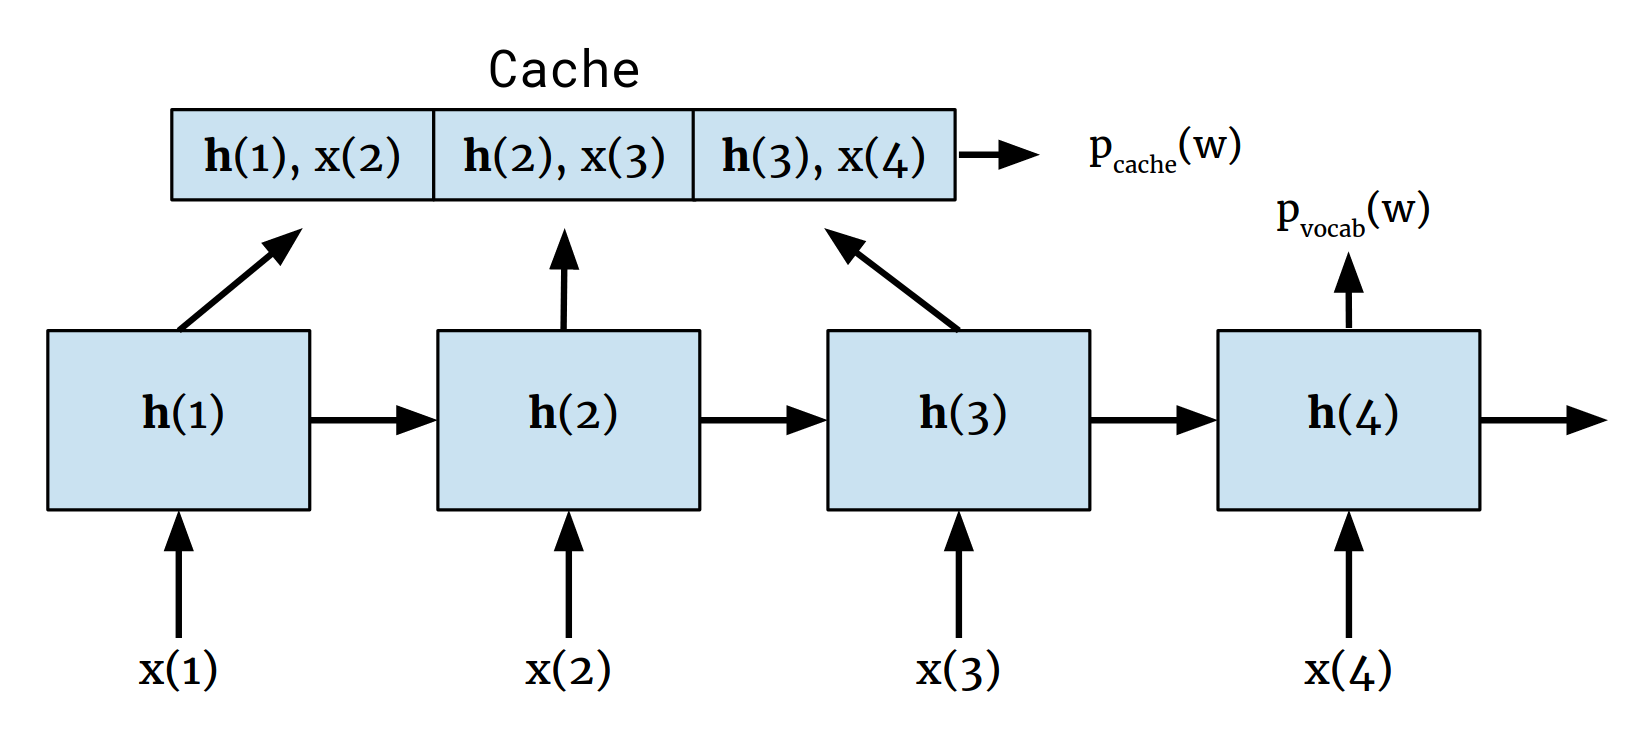
\includegraphics[scale=0.2]{cache}
	\captionof{figure}{Neural Continuous Cache Model.}
	\label{fig:cache}
\end{figure}

Each hidden representation $\mathbf{h}(i)$ acts as the key of each cache entry, which contains the word $x(i+1)$ (the correct output for timestep $i$). Furthermore, the hidden representations are exploited to define a probability distribution over the words in the cache; at timestep $t$, the probability for each word in the cache is expressed as:

\begin{equation} \label{eq:cacheProb}
	p_{\text{cache}}(w|\mathbf{h}(1\ldots t)) = \sum_{i=1}^{t-1} \mathbb{1}_{w=x(i+1)} e^{\theta\mathbf{h}(t)^{\top}\mathbf{h}(i)}
\end{equation}

where $\mathbf{h}(1\ldots t)$ represents the sequence of hidden states for times $1$ to $t$ and $\theta \in \mathbb{R}$ controls the sharpness of the distribution ($\theta=0$ would lead to a uniform distribution over all the words in the cache).

It can be observed that this formulation resembles the one from the attention models that we have introduced in the previous sections. The ``score'' of each word in the cache is obtained as the dot product $\mathbf{h}(t)^{\top}\mathbf{h}(i)$ (it is worth noting that this scoring mechanism doesn't require any parametrization). The distribution $p_{\text{cache}}(w)$ is then obtained by normalizing these scores with a softmax. To obtain the final output probability of the model, we blend the cache distribution with our usual vocabulary distribution (probabilities for all the words contained in the vocabulary) by means of linear interpolation:

\begin{equation} \label{eq:contCache}
	p(w|\mathbf{h}(1\ldots t)) = (1-\lambda)p_{\text{vocab}}(w|\mathbf{h}(t)) + \lambda p_{\text{cache}}(w|\mathbf{h}(1\ldots t))
\end{equation}

where $\lambda$ is a fixed hyperparameter that controls the linear interpolation weight of each distribution and is chosen by optimizing performance on a validation set. 

In summary, the neural continuous cache constitutes a simple yet powerful technique for RNNLMs to adapt to the recent history of words. By design, it doesn't require to be trained and thus, it can be applied on top of any pretrained model using big cache sizes.

\section{Pointer Sentinel Mixture Model (PSMM)}
\label{sec:pointerMixture}

Presented in \cite{merity2016pointer}, this model is characterized by the introduction of a pointer component (inspired by pointer networks \cite{vinyals2015pointer}) in addition to the usual vocabulary softmax. As we will see, this is equivalent to the neural continuous cache detailed in \autoref{sec:continuousCache}. However the main difference lies in the fact that the interpolation weight is dynamically calculated, allowing the model to learn when to use each component. Similar to pointer networks, the pointer component keeps track of the previous inputs. However rather than directly outputting one of the previous inputs (as pointer networks do), the pointer component produces a probability distribution over them as illustrated in \autoref{fig:psmm}.

\begin{figure}[H]
	\centering
	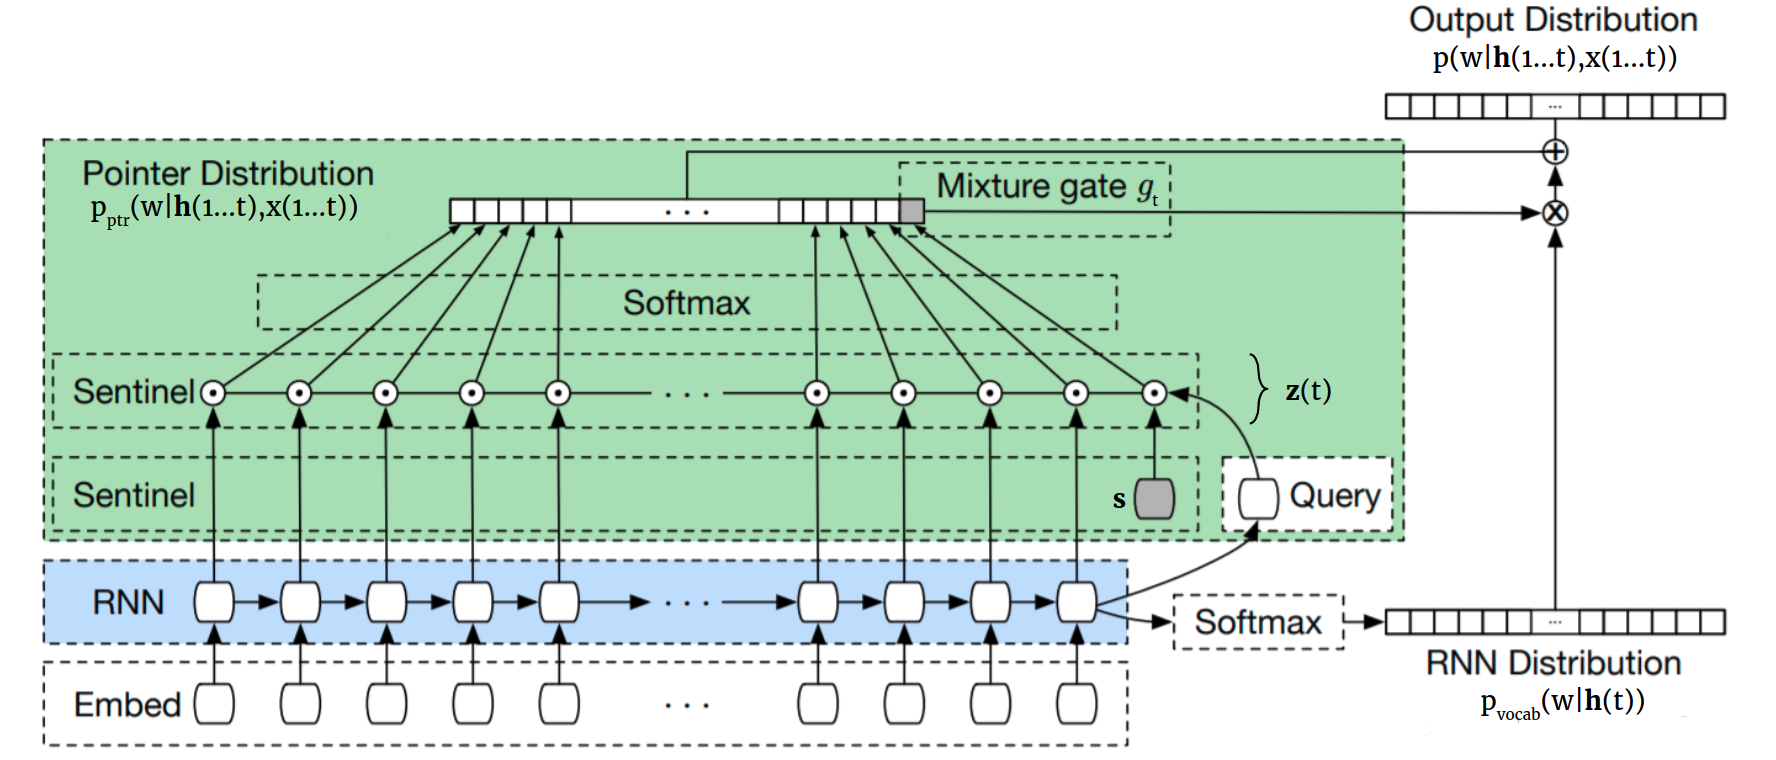
\includegraphics[scale=0.22]{psmm}
	\captionof{figure}{Pointer Sentinel Mixture Model architecture \cite{merity2016pointer}.}
	\label{fig:psmm}
\end{figure}

Given an input $x$ that consists of the sequence $\{w_1, \cdots , w_t\}$ of input word IDs up to $t$ and $y(t)$ the ID of the correct word that has to be predicted $w_{t+1}$, in theory the pointer component would take into account the whole input. In practice due to memory limitations only a window of the $L$ most recent words is  for the pointer to match against. Thus both the hidden states and the respective word IDs inside the window need to be stored, as shown in \autoref{eq:psmmMemory}.

\begin{equation} \label{eq:psmmMemory}
	\begin{gathered}
		M(t) = [\mathbf{h}(t); \cdots; \mathbf{h}(t-L+1) ] \\
		\mathbf{m}(t) = [w_t; \cdots; w_{t-L+1}] \\
	\end{gathered}
\end{equation}

where $M(t) \in \mathbb{R}^{H \times L}$ and $\mathbf{m}(t) \in \mathbb{R}^{L}$. 

In order to obtain the attention scores $\mathbf{z}(t)$ over the window, the easiest way is to compute the dot product between the current hidden state $\mathbf{h}(t)$ and all the hidden states in the window (like in \autoref{sec:continuousCache}). However the window also contains $\mathbf{h}(t)$ as this word may be repeated ($w_{t+1}$ is equal to $w_t$), and as the dot product of a vector with itself results in its magnitude squared, the attention scores would be biased towards the last word. Therefore the authors chose to avoid this by projecting $\mathbf{h}(t)$ into a query vector $\mathbf{q}(t)$ (\autoref{eq:psmmScores}).

\begin{equation} \label{eq:psmmScores}
	\begin{gathered} 
		\mathbf{q}(t) = \tanh(W\mathbf{h}(t) + \mathbf{b}) \\
		\mathbf{z}(t) = \mathbf{q}(t)^{\top} M(t)
	\end{gathered}
\end{equation}

where $\mathbf{q}(t),\mathbf{b} \in \mathbb{R}^{H}$, $W \in \mathbb{R}^{H \times H}$ and $\mathbf{z}(t) \in \mathbb{R}^{L}$. 

As mentioned at the beginning of this section, the weight for interpolating both components is calculated dynamically at each timestep. To do this, a trainable sentinel vector $\mathbf{s}$ is also multiplied with the query vector to obtain the score for using the vocabulary component rather than the pointer. Once we normalize with the softmax, we obtain the gate $g_t$ that will weight the two components:

\begin{equation} \label{eq:psmmSentinel}
	\begin{gathered} 
		\mathbf{a}(t) = \text{softmax}([\mathbf{z}(t); \mathbf{q}(t)^{\top} \mathbf{s}]) \\
		g_t = \mathbf{a}(t)_{L+1}
	\end{gathered} 
\end{equation}

where $\mathbf{a}(t) \in \mathbb{R}^{L+1}$, $\mathbf{s} \in \mathbb{R}^{h}$ and $g_t \in \mathbb{R}$.

It can be seen in \autoref{eq:psmmSentinel} that the values $\mathbf{a}(t)_{1:L}$ correspond to the pointer probabilities where the probability mass assigned to $g_t$ has been subtracted from the pointer. Hence, the final normalized pointer probabilities are:

\begin{equation}
	\begin{gathered}
		p_{\text{ptr}}(w|\mathbf{h}(1\ldots t)) = \frac{1}{1-g_t}\mathbf{a}(t)_{1:L} \\
		p_{\text{ptr}}(w=i|\mathbf{h}(1\ldots t)) = \frac{1}{1-g_t}\sum_{k \in I(i, \; \mathbf{m}(t))}\mathbf{a}(t)_k \; \in \; \mathbb{R}
	\end{gathered}
\end{equation}

where $p_{\text{ptr}}(w|\mathbf{h}(1\ldots t)) \in \mathbb{R}^{L}$, $p_{\text{ptr}}(w=i|\mathbf{h}(1\ldots t)) \in \mathbb{R}$ and $I(i, \; \mathbf{m}(t))$ results in all positions of $\mathbf{m}(t)$ (the window of previous word IDs) that are equal to $i$.

Once the pointer probabilities and the gate have been calculated, the output distribution is obtained as:

\begin{equation}
	\begin{gathered}
		p(w=i|\mathbf{h}(1\ldots t)) = g_t \, p_{\text{vocab}}(w=i|\mathbf{h}(t)) + (1-g_t) \, p_{\text{ptr}}(w=i|\mathbf{h}(1\ldots t)) \\
		= g_t \, p_{\text{vocab}}(w=i|\mathbf{h}(t)) + \sum_{k \in I(i, \; \mathbf{m}(t))}\mathbf{a}(t)_k
	\end{gathered}
\end{equation}

The loss function used to optimize the model (\autoref{eq:psmmLoss}) is made up of two parts: the first one is the traditional cross-entropy loss used in RNNLMs. An intuitive explanation for the second part is that it supervises the pointer component and makes sure that if any probability mass is taken from the vocabulary softmax and given to the pointer, it was the right thing to do (i.e. the correct output $y(t)$ appears one or more times in the window and the pointer assigns its probability to these positions).

\begin{equation} \label{eq:psmmLoss}
	\begin{gathered}
		\mathcal{L}(\theta) = -\log(p(w=y(t)|\mathbf{h}(1\ldots t)) -\log(g_t + \sum_{i \in I(y(t), \; x(t))}\mathbf{a}(t)_i) \\
		= -\log(g_t \, p_{\text{vocab}}(w=y(t)|\mathbf{h}(1\ldots t)) + \sum_{k \in I(y(t), \; x(t))}\mathbf{a}(t)_k) \\
		-\log(g_t + \sum_{i \in I(y(t), \; x(t))}\mathbf{a}(t)_i)
	\end{gathered}
\end{equation}

\section{Our approach: Softmax Mixture Model (SMM)}
\label{sec:mixtureModel}

To conclude this chapter we introduce our proposed model called the ``Softmax Mixture''. Inspired by the models detailed in the previous sections, we also use two components that are blended with a dynamically calculated weight. In our case both components are of the same type, softmax distributions over the whole vocabulary (as in \autoref{sec:rnn}).

Similar to \cite{gulcehre2016pointing}, we define a binary variable $z_t$ that indicates which distribution (out of two)  produced the output word. Then, a switching network that takes as input the current hidden state $\mathbf{h}(t)$ outputs a scalar probability $p(z_t=1|\mathbf{h}(t))$:

\begin{equation} \label{eq:probSwitch}
	p(z_t=1|\mathbf{h}(t)) = \sigma(f(\mathbf{h}(t);\theta))
\end{equation}

where $\sigma(\cdot)$ is the sigmoid function and $f(\cdot)$ is a multilayer perceptron.

This probability is then used as the interpolation weight that controls the blending of the two distributions. With this architecture we want to fulfill two objectives: be able to distinguish the correct source of each word (by means of the supervised switching network) and fit two differentiated output distributions that match the characteristics of each source. 

\begin{equation} \label{eq:smm}
	\begin{gathered}
		p(w|\mathbf{h}(t)) = p(z_t=1|\mathbf{h}(t))p(w|\mathbf{h}(t), z_t=1) \\
		+ (1-p(z_t=1|\mathbf{h}(t)))p(w|\mathbf{h}(t), z_t=0)
	\end{gathered}
\end{equation}

Finally, in addition to the cross-entropy loss term used to optimize the RNNLM we introduce the sigmoid cross-entropy loss of the switching network to train it in a supervised fashion, as shown in \autoref{eq:smmLoss}.

\begin{equation} \label{eq:smmLoss}
	\begin{gathered}
		\mathcal{L}(\theta) = -\log(p(w|\mathbf{h}(t))) \\
		- \lambda(z_t\log(p(z_t=1|\mathbf{h}(t))) + (1 - z_t)\log(p(z_t=0|\mathbf{h}(t)))
	\end{gathered}
\end{equation}

where $\lambda$ is a hyperparameter that controls how much weight is given to the switch network loss.
